\documentclass{article}
\usepackage[utf8]{inputenc}
\usepackage[a4paper, total={7in, 9in}]{geometry}
\usepackage{minted}
\usepackage{graphicx}
\usemintedstyle{manni}

\title{HPC 4}
\author{dinhanhx }
\date{December 2022}

\begin{document}

\maketitle

\section{Implementation}

\begin{figure}[htbp]
    \centering
    
\includegraphics[scale=0.8]{gura.png}
    \caption{RGB Gura image}
    \label{fig:rgb}
\end{figure}

\begin{figure}[htbp]
    \centering
    
\includegraphics[scale=0.2]{gray_gura.png}
    \caption{Gray Gura image}
    \label{fig:gray}
\end{figure}

\subsection{CPU}

\begin{minted}{python}
def rgb2gray(src, dst):
    for i in range(src.shape[0]):
        for j in range(src.shape[1]):
            g = (int(src[i, j, 0]) + int(src[i, j, 1]) + int(src[i, j, 2])) / 3
            dst[i, j, 0] = dst[i, j, 1] = dst[i, j, 2] = g
\end{minted}

So here I use a for loop which updates each triplet (RGB) by taking the average of them.

\subsection{GPU}

\begin{minted}{python}
@cuda.jit
def rgb2gray(src, dst):
    i = cuda.threadIdx.x + cuda.blockIdx.x * cuda.blockDim.x
    ii = cuda.threadIdx.y + cuda.blockIdx.y * cuda.blockDim.y
    g = np.uint8((src[i, ii, 0] + src[i, ii, 1] + src[i, ii, 2]) / 3)
    dst[i, ii, 0] = dst[i, ii, 1] = dst[i, ii, 2] = g
\end{minted}

So here I use \mintinline{python}{@cuda.jit} and get the current coordinate (x, y) of block and thread that kernel function is working with.

\section{Block size vs time}

\begin{figure}[htbp]
    \centering
    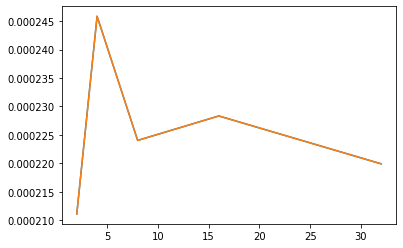
\includegraphics[scale=0.8]{block_size_vs_time.png}
    \caption{Block size vs time}
    \label{fig:block_size_vs_time}
\end{figure}

I have no comments

\end{document}
